\section{Evaluation}


In this section, we evaluate the proposed optimization, where we analyze our
improvements on code size reduction, as well as its impact on the program's
performance and compilation-time.



\subsection{Experimental Setup}
We compare our optimization against the state-of-the-art function merging approach of Edler von Koch et al.~\cite{edler14} and LLVM's identical
function merging. In our evaluation, we refer to identical function merging as \textit{Identical}, the state-of-the-art as \textit{SoA}, and our
approach as \textit{FMSA}.

All optimizations are implemented in LLVM v7 and evaluated on the C/C++ SPEC CPU2006~\cite{spec} benchmark suite. We target two different
instruction sets, the Intel x86-64 and the ARM Thumb. Our Intel testbench has a quad-core 3.4~GHz Intel Core i7 CPU with 16~GiB of RAM.
%The operating system is openSUSE 42.2 with Linux kernel version 4.4.27.
The ARM testbench has a Cortex-A53 ARMv8 CPU of 1.4~GHz with 1~GiB of RAM.
%The operating system of the ARM platform is a Raspbian.
We use the Intel platform for compiling for either target. As a result, compilation-time is almost
identical for both targets. Changing the target only affects the behavior of the backend, a very
short part of the pipeline. Because of that, we only report compilation-time overhead results for
one of the targets, the Intel ISA.

\begin{figure*}[t!]
  \centering
  %\subfigure[Intel platform.]{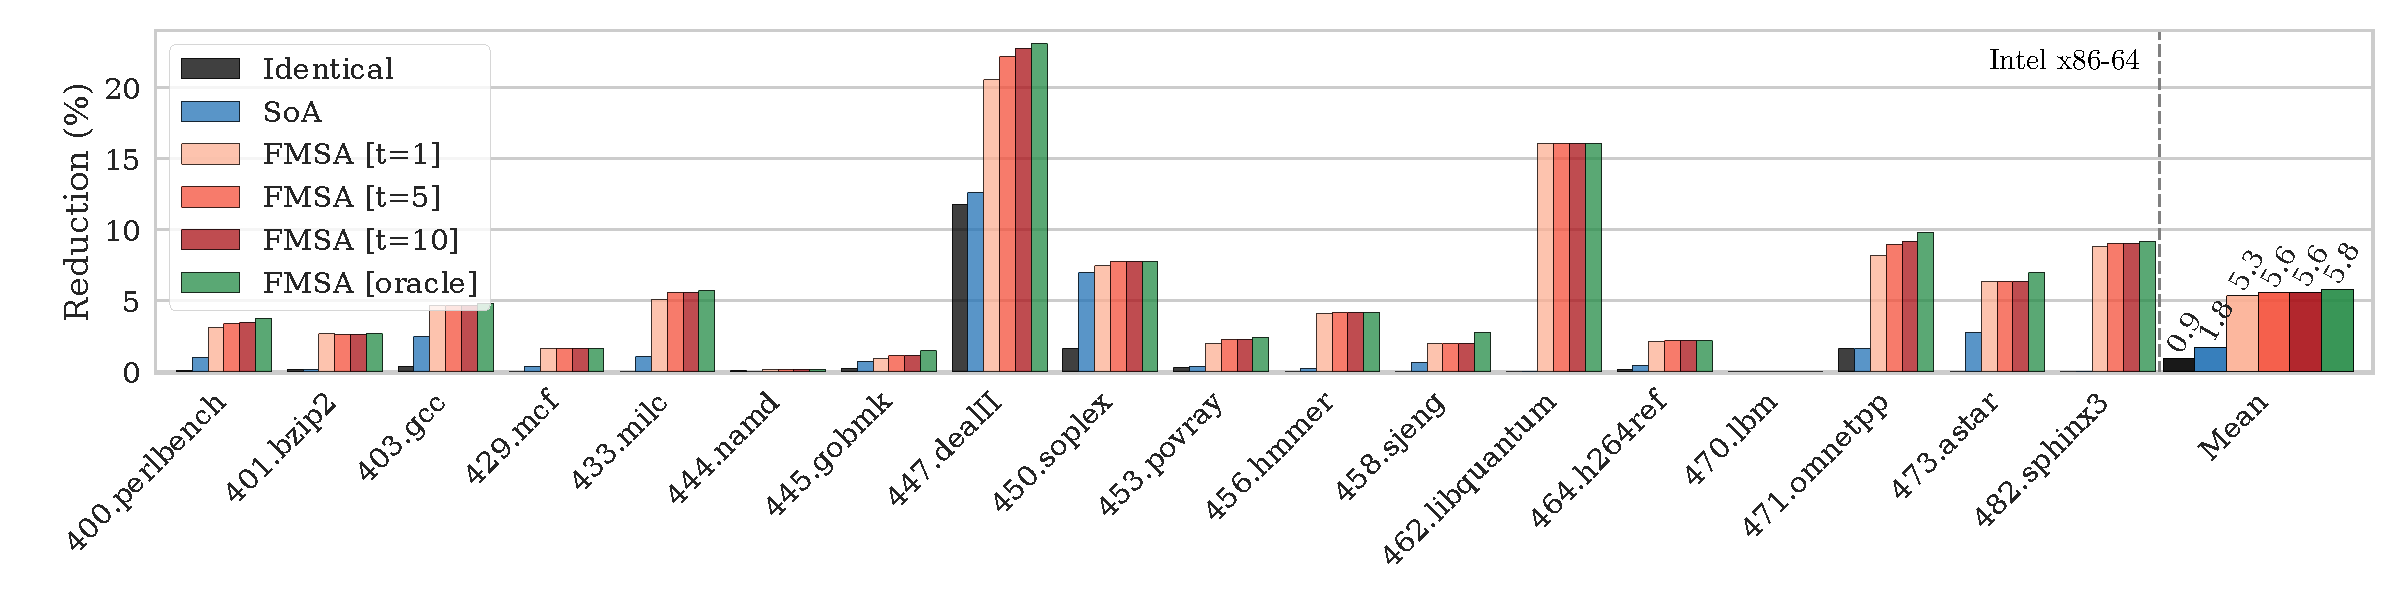
\includegraphics[width=\linewidth]{figs/reduction-obj-intel-label.pdf}}
  %\subfigure[ARM platform.]{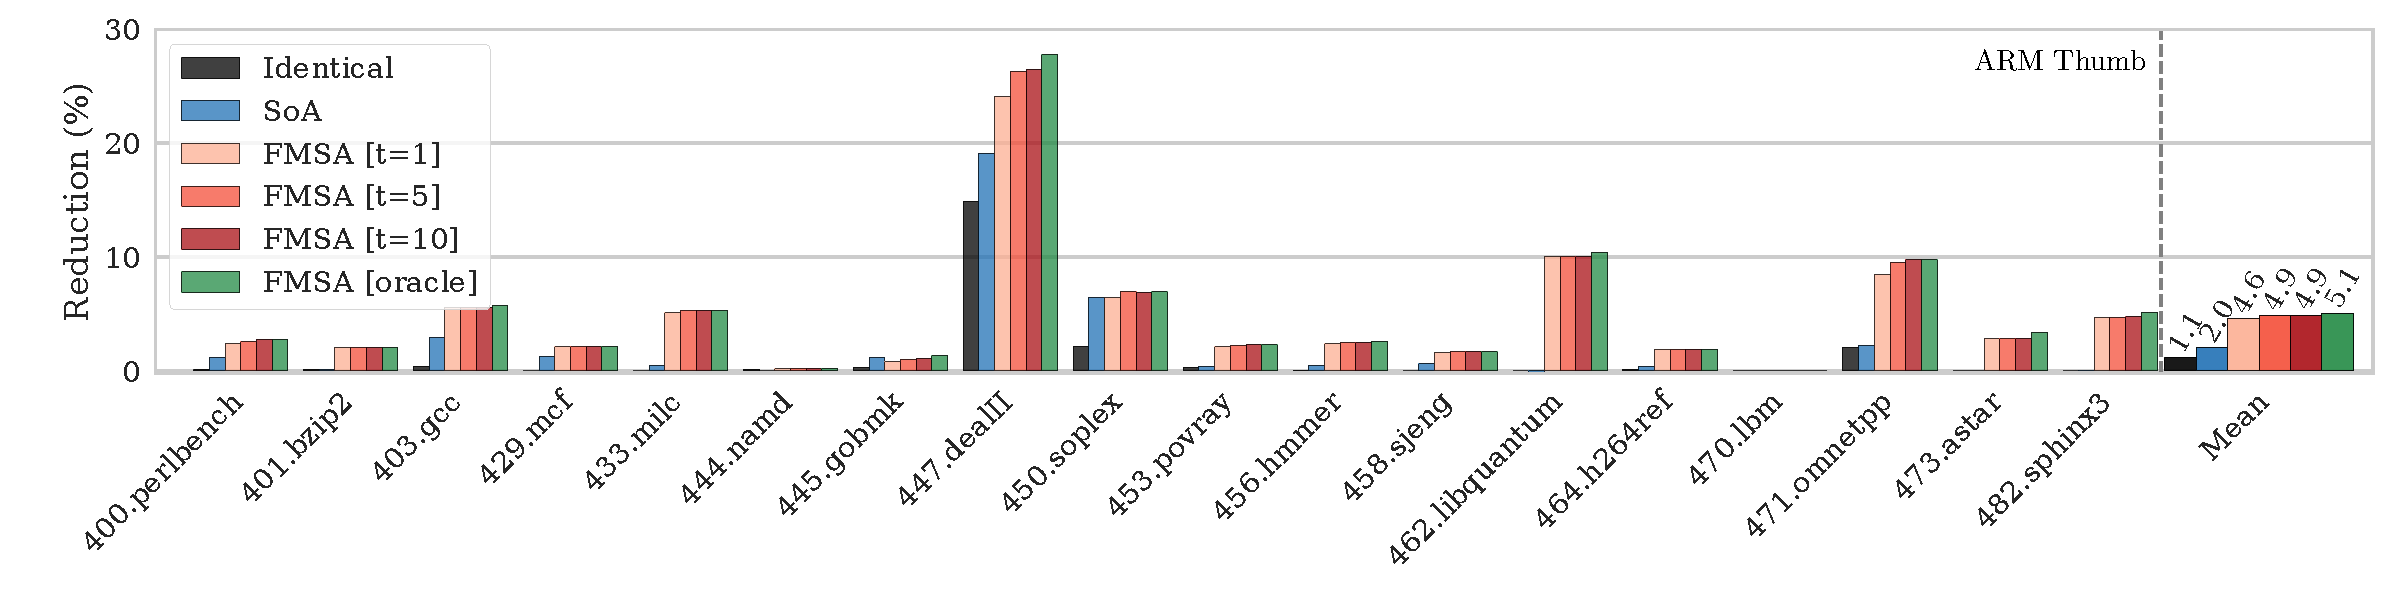
\includegraphics[width=\linewidth]{figs/reduction-obj-arm-label.pdf}}
  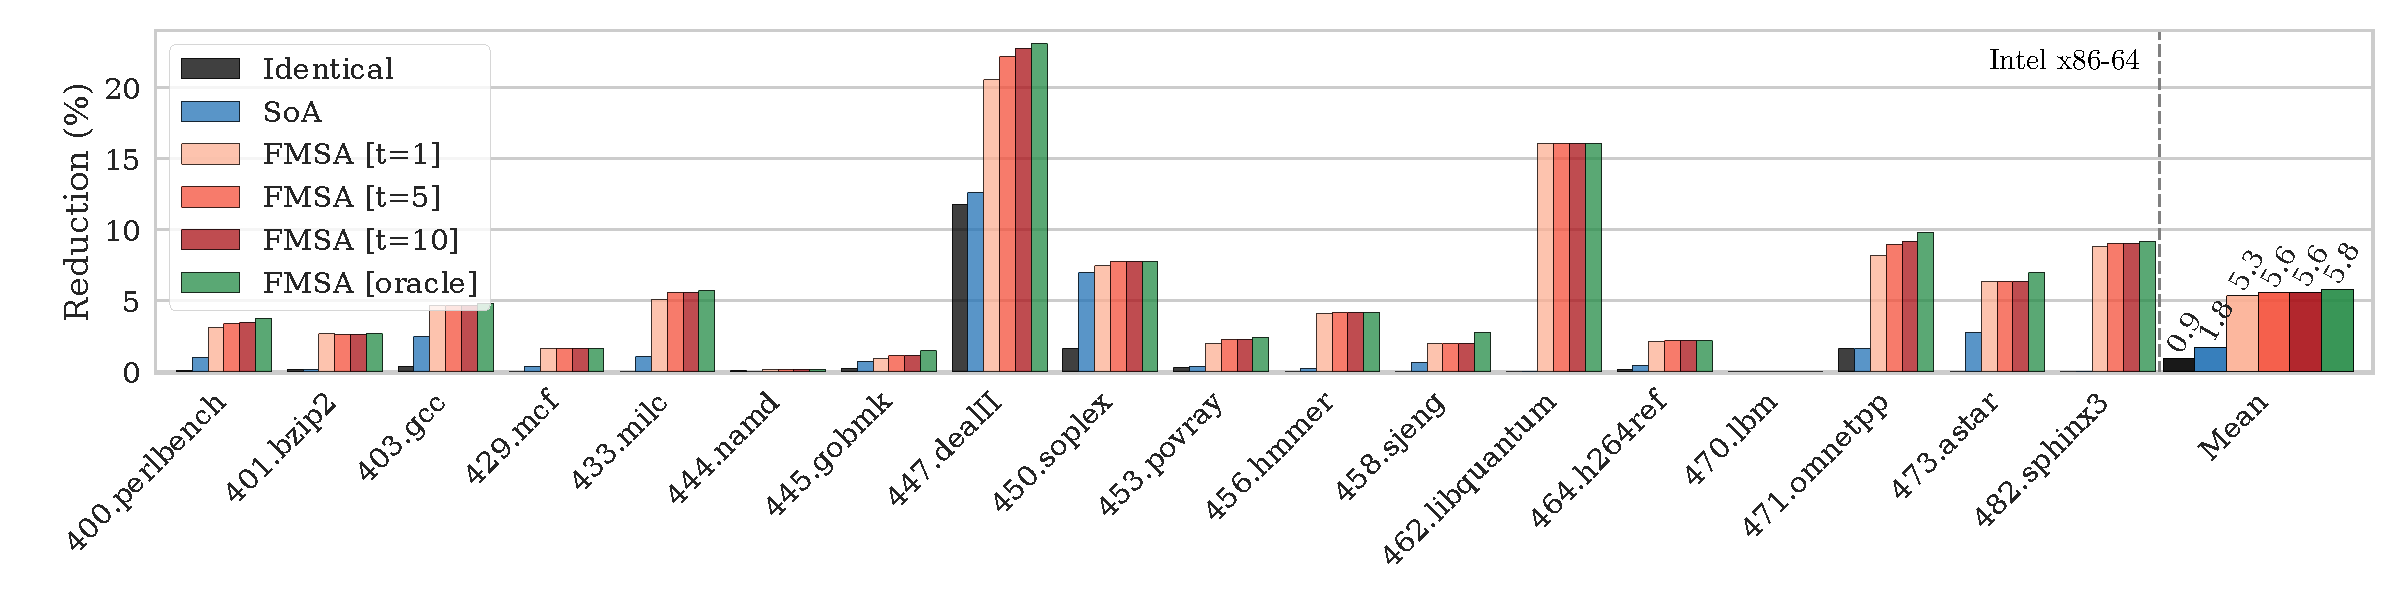
\includegraphics[width=\linewidth]{figs/reduction-obj-intel-label.pdf} \\
  \vspace{-1.8ex}
  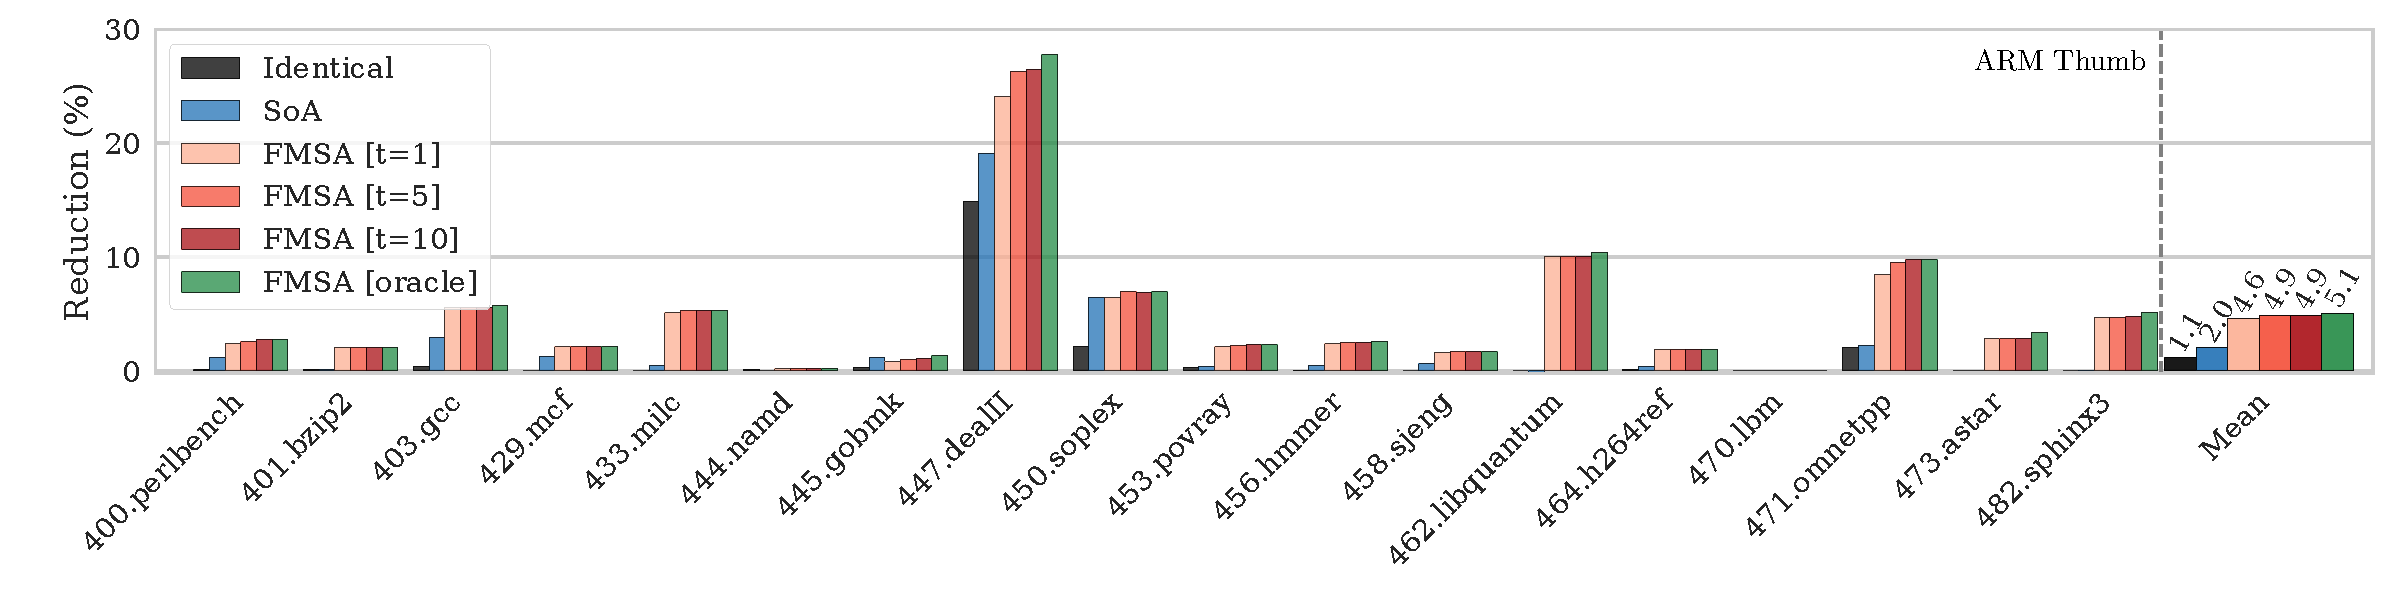
\includegraphics[width=\linewidth]{figs/reduction-obj-arm-label.pdf}
  \vspace{-4ex}
	\caption{Object file size reduction for Intel (top) and ARM (bottom). We evaluate our approach (FMSA) under four different exploration thresholds, which
      control how many potential merging pairs we examine for each function before making a decision. Even for a threshold of one, we outperform the state-of-the-art
	  by 2.9$\times$(Intel) and 2.3$\times$ (ARM).}
  \label{fig:reduction-obj}
\end{figure*}

For the proposed optimization, we vary the exploration threshold (Section~\ref{sec:framework})
and we present the results for a range of threshold values. We also show the results for the oracle exploration strategy, which
instead of using a rank-based greedy approach, merges a function with all candidates and chooses the best one.
%The oracle represents the results assuming a perfect ranking strategy.
%However, the oracle has a very costly quadratic exploration, as explained in
%Section~\ref{sec:framework}.
This oracle is a perfect ranking strategy but is unrealistic. It requires a very costly quadratic exploration, as explained in
Section~\ref{sec:framework}. \fixme{ZW: I suggest we call ``oracle" exhaustive-exploration instead. ``oracle" is often used to refer the
up-bound performance.}



\subsection{Code-Size Reduction}

%\begin{figure*}[th]
%  \centering
%  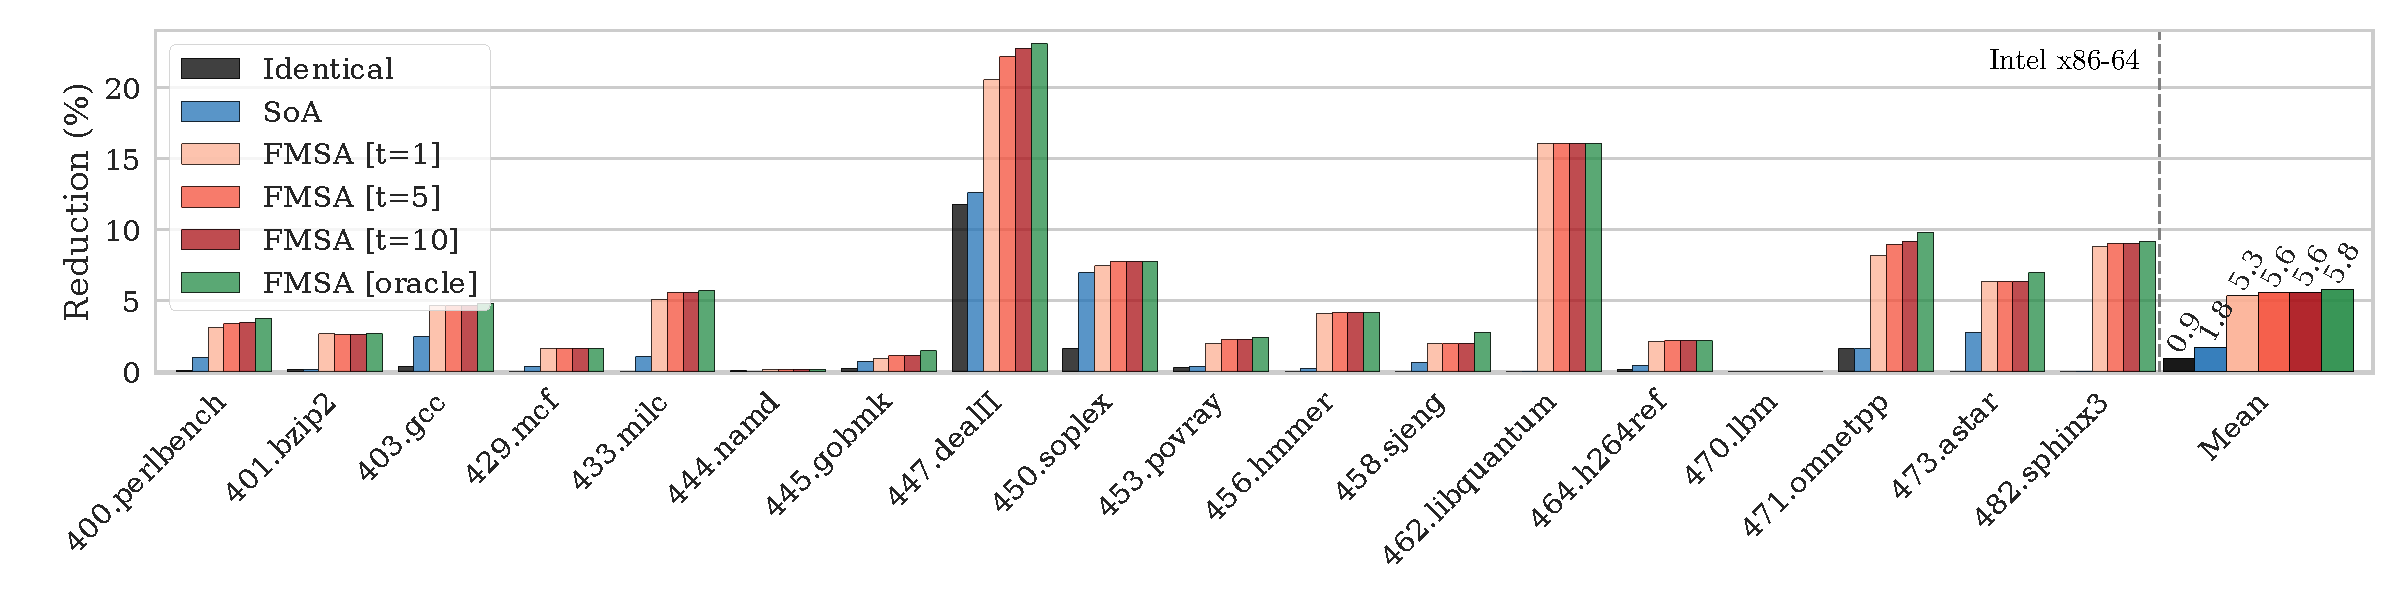
\includegraphics[width=\linewidth]{figs/reduction-obj-intel-label.pdf}
%  \caption{Reduction on the object file for the Intel architecture.}
%  \label{fig:reduction-obj-intel}
%\end{figure*}
%\begin{figure*}[th]
%  \centering
%  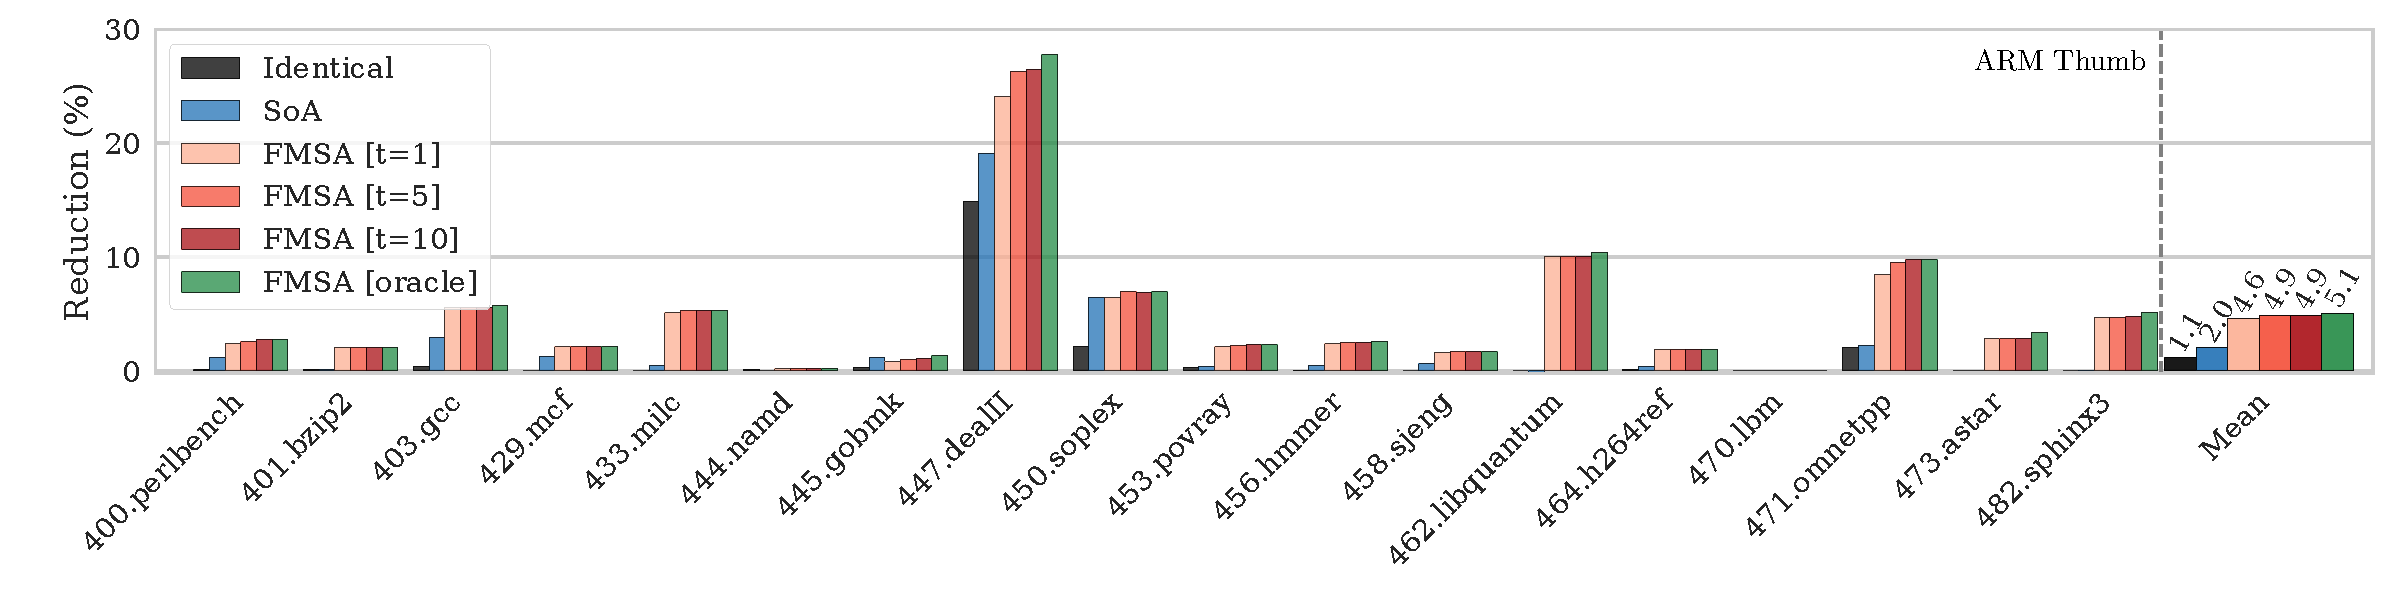
\includegraphics[width=\linewidth]{figs/reduction-obj-arm-label.pdf}
%  \caption{Reduction on the object file for the ARM architecture.}
%  \label{fig:reduction-obj-arm}
%\end{figure*}


Figure~\ref{fig:reduction-obj} reports the code size reduction over the baseline for the linked object. %These results show how much we can improve over the existing techniques, by having a more powerful solution, and how close we
%can get to the oracle with our ranking-based exploration framework.
We observe similar trends of code size reduction on both target architectures. This is expected because the
optimizations are applied at the platform-independent IR level. Changing the target architecture introduces only second order effects,
such as slightly different decisions due to the different cost model (LLVM's TTI) and differences in how the IR is encoded into binary.

Our approach, FMSA, significantly improves over the state-of-the art (SoA). For the Intel platform, FMSA can achieve an average code size
reduction of up to 5.8\% (or 5.3\% with the lowest exploration threshold), while the SoA and Identical had an average reduction of 1.8\% and 0.9\%,
respectively. Similarly, for the ARM platform, FMSA can achieve an average code size reduction of up to 5.1\% (or 4.6\% with the lowest
threshold), while SoA and Identical had an average reduction of 2\% and 1.1\%, respectively. For several of the benchmarks, the
proposed technique achieves impressive code size reduction compared to other merging approaches. Table~\ref{tab:reduction} highlights
some of these results for both platforms. In two cases, \texttt{462.libquantum} and \texttt{482.sphinx3}, the state-of-the-art slightly
increases code size, while FMSA shows reduces size significantly.  The only case where SOA outperforms FMSA is on the \texttt{445.gobmk}
benchmark on the ARM platform. There are little opportunities for function merging on that benchmark and FSMA misses a few of them. 
However, we can easily fix this by increasing the exploration threshold. For exhaustive exploration, FMSA improves over the SoA,
with a code size reduction of 1.33\%. In all other cases, FMSA is always equal or better than all other function-merging optimizations, usually by a significant margin.

\begin{table}[]
\label{tab:reduction}
\centering
\scalebox{0.8}{
\begin{tabular}{lccc}
\toprule
\multicolumn{1}{c}{\textbf{Benchmarks}} & \textbf{Identical} & \textbf{SoA}  & \textbf{FMSA {[}t=1{]}} \\
\midrule
%%%400.perlbench                             & 0.09 / 0.09        & 1.03 / 1.15   & 3.13 / 2.40             \\ \hline
\rowcolor{evencolor} 401.bzip2                                 & 0.15 / 0.16        & 0.15 / 0.16   & 2.67 / 2.09             \\
%%%403.gcc                                   & 0.36 / 0.43        & 2.48 / 2.89   & 4.71 / 5.59             \\ \hline
%%%429.mcf                                   & 0 / 0              & 0.41 / 1.29    & 1.66 / 2.11             \\ \hline
433.milc                                  & 0 / 0              & 1.08 / 0.46   & 5.09 / 5.12             \\
%%%444.namd                                  & 0.10 / 0.14        & 0 / 0         & 0.20 / 0.17             \\ \hline
\rowcolor{evencolor} 447.dealII                                & 11.77 / 14.83      & 12.59 / 19.12 & 20.57 / 24.08           \\
445.gobmk                                 & 0.26 / 0.32        & 0.77 / 1.15   & 0.96 / 0.78             \\
%%%450.soplex                                & 1.62 / 2.16        & 6.99 / 6.47   & 7.46 / 6.48             \\ \hline
\rowcolor{evencolor} 453.povray                                & 0.28 / 0.33        & 0.38 / 0.40   & 2.04 / 2.12             \\
456.hmmer                                 & 0 / 0              & 0.27 / 0.50   & 4.15 / 2.40             \\
%%%458.sjeng                                 & 0 / 0              & 0.63 / 0.63   & 1.97 / 1.62             \\ \hline
\rowcolor{evencolor} 462.libquantum                            & 0 / 0              & -0.07 / -0.17 & 16.08 / 10.04           \\
%%%464.h264ref                               & 0.16 / 0.14        & 0.47 / 0.40   & 2.16 / 1.86             \\ \hline
%%%470.lbm                                   & 0 / 0              & 0 / 0         & 0 / 0                   \\ \hline
471.omnetpp                               & 1.65 / 2.08        & 1.64 / 2.27   & 8.18 / 8.47             \\
\rowcolor{evencolor} 473.astar                                 & 0 / 0              & 2.76 / 0      & 6.33 / 2.81             \\
482.sphinx3                               & 0 / 0              & -0.06 / 0.06  & 8.85 / 4.72             \\
\bottomrule
\end{tabular}
}
\caption{Highlights of code reduction results (in percentages) on \textit{Intel / ARM} platforms. }
\end{table}

In most cases, LLVM's identical function merging has very little impact on code size. We see noticeable impact
only on some of the C++ benchmarks, namely, \texttt{447.dealII}, \texttt{450.soplex}, and \texttt{471.omnetpp}.
These are the cases that identical function merging was designed to handle, duplicate functions due to heavy
use of templating. But even on these benchmarks FMSA outperforms LLVM, with an improvement of almost 6$\times$
on the \texttt{471.omnetpp} benchmark. FMSA will by design merge a superset of the functions LLVM would merge,
so it will never produce a worse result. Moreover, our technique also shows remarkable reductions on several of the C benchmarks, such as, \texttt{462.libquantum} and
\texttt{482.sphinx3}, where other techniques have no real impact.

%Figure~\ref{fig:libquantum-example} shows an example of two functions\footnote{We
%have changed very lightly some of the names used in the functions so that the
%code fits nicely in the paper. The original names of the functions are:
%quantum\_cond\_phase and quantum\_cond\_phase\_inv.}
%from the 462.libquantum benchmark that are merged by the proposed optimization.
%The proposed function-merging technique is the \textit{first} technique able to
%merge these two functions.
%Although they are very similar functions, the state-of-the-art is unable to
%merge them since their CFGs are not structurally identical.
%For the proposed optimization, however, these two functions receive a similarity
%score above $0.49$, which puts them at the top of the rank, and the
%profitability cost model estimates a code-size reduction of 40\%.
%Overall, our optimization was able to merge nine pairs of functions for the
%462.libquantum benchmark.
%Similar to the example shown, all of them were top ranked based on their
%fingerprint similarity.

%Note that functions that are identical at the IR or machine level are not
%necessarily identical at the source level.
%Figure~\ref{fig:identical-example} shows two real functions extract from the
%447.dealII program in the SPEC CPU2006~\cite{spec} benchmark suite.
%Although these two functions are not identical at the source level, they become
%identical after a template specialization and some optimizations are applied, in
%particular, constant propagation, constant folding, and dead-code elimination.
%Specializing \verb|dim| to $1$ enables to completely remove the loop in the
%function \verb|PolynomialSpace|.
%Similarly, specializing \verb|dim| to $1$ results in only the first iteration
%of the loop in the function \verb|TensorProductPolynomials| being executed.
%The compiler is able to statically analyze and simiplify the loops in both
%functions, resulting in the identical functions shown at the bottom of
%Figure~\ref{fig:identical-example}.


%\begin{figure*}[t]
%  \centering
%  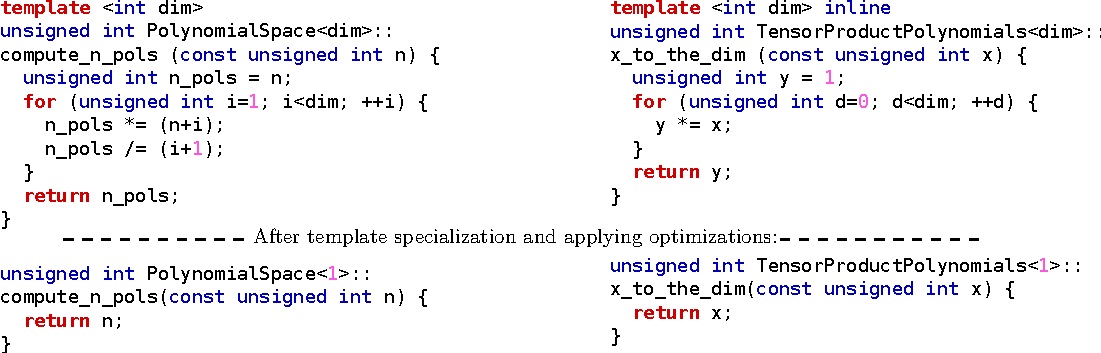
\includegraphics[width=0.95\linewidth]{figs/identical-example.pdf}
%  \caption{Two function extracted from the 447.dealII benchmark that are not
%           identical at the source level, but after applying template
%           specialization and optimizations they become identical at the IR
%           level.}
%  \label{fig:identical-example}
%\end{figure*}


\subsection{Compilation Overhead}

\begin{figure*}[t]
  \centering
  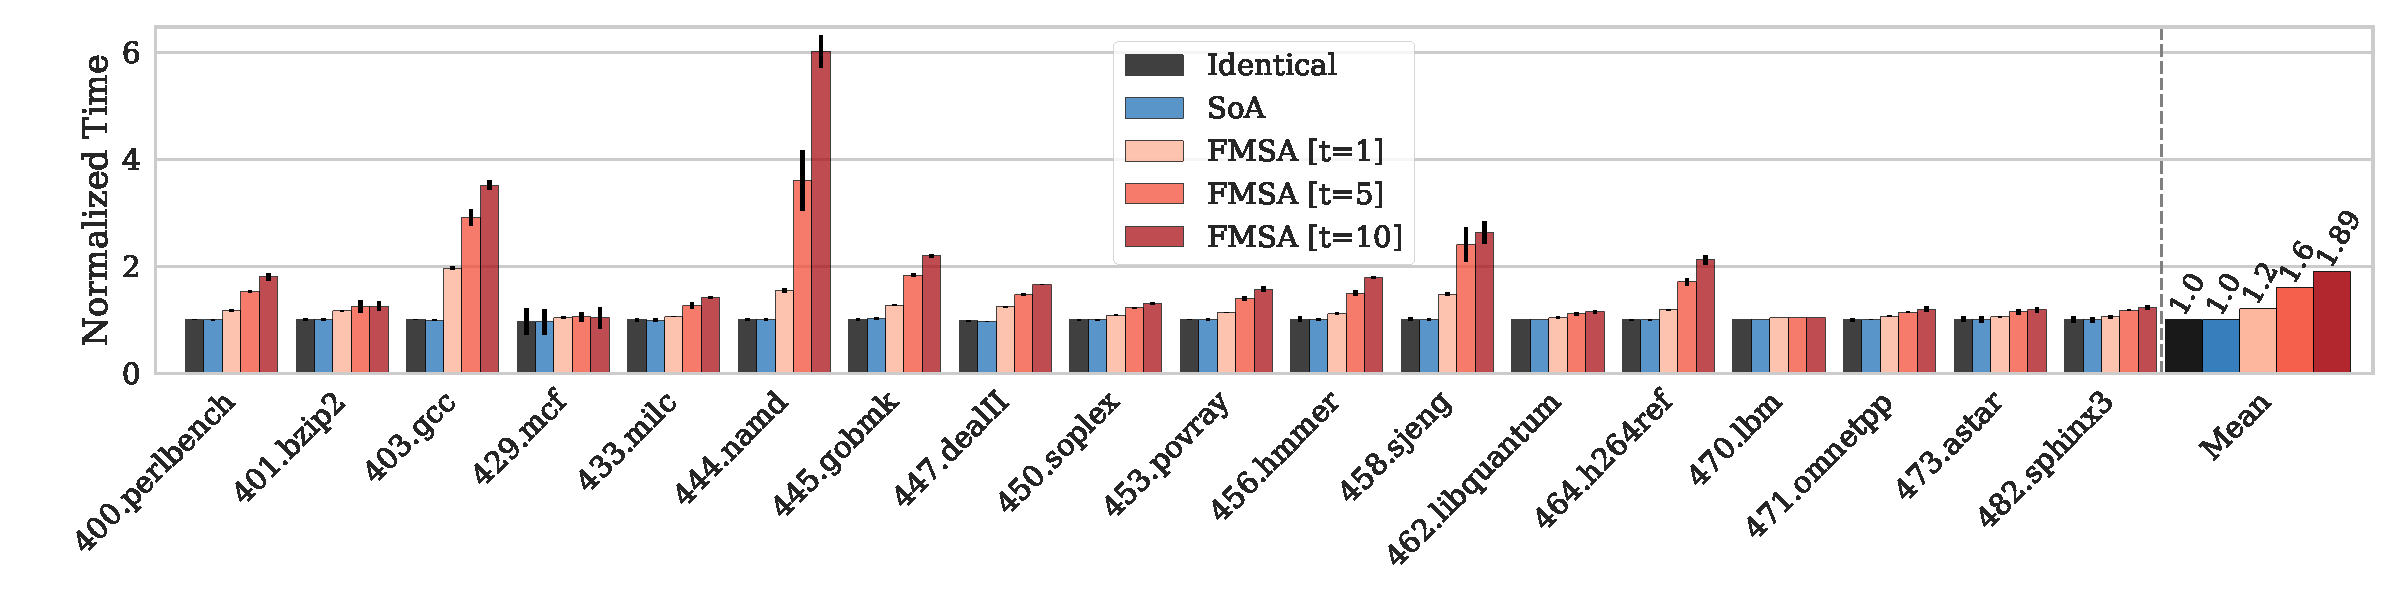
\includegraphics[width=\linewidth]{figs/compilation-time.pdf}
  \vspace{-4ex}
	\caption{Compilation-time overhead on the Intel platform. For an exhaustive exploration (not shown) the average overhead is 25$\times$. Through ranking, we reduce the overhead by orders of magnitude. For an exploration threshold of one, FMSA has an overhead of only 20\%.}
  \label{fig:compilation-time}
\end{figure*}


Figure~\ref{fig:compilation-time} shows the compilation-time overhead for all
optimizations.
As explained in the experimental setup, we only present results for compiling
for Intel. Since we cross-compile on the same machine for both targets, compilation
times are very similar. We also do not include results for the oracle (exhaustive) exploration.
It would be hard to visualize it in the same plot as the other configurations, since it
can be up to 136$\times$ slower than the baseline.

\begin{figure}[t]
  \centering
  %\hspace{-2ex}
  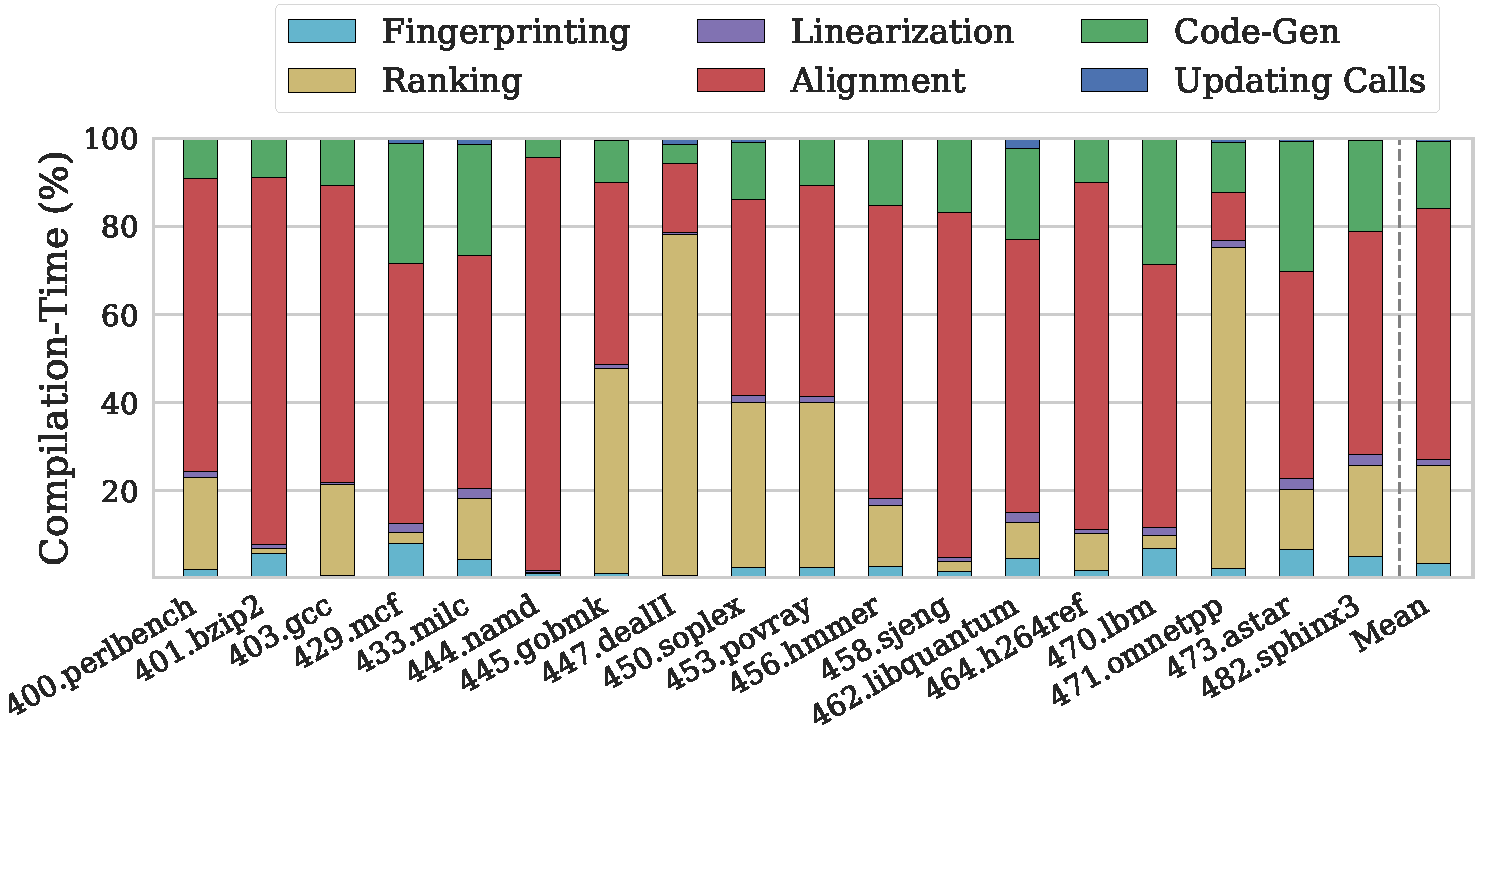
\includegraphics[width=1.0\linewidth]{figs/compilation-time-breakdown-sqrd.pdf}
  \vspace{-8.5ex}
  \caption{A compilation-time breakdown isolating the percentage for each major
           step of the optimization (t=1).}%, with an exploration threshold of one.}
  \label{fig:compilation-time-breakdown}
\end{figure}

\begin{figure*}[t]
  \centering
  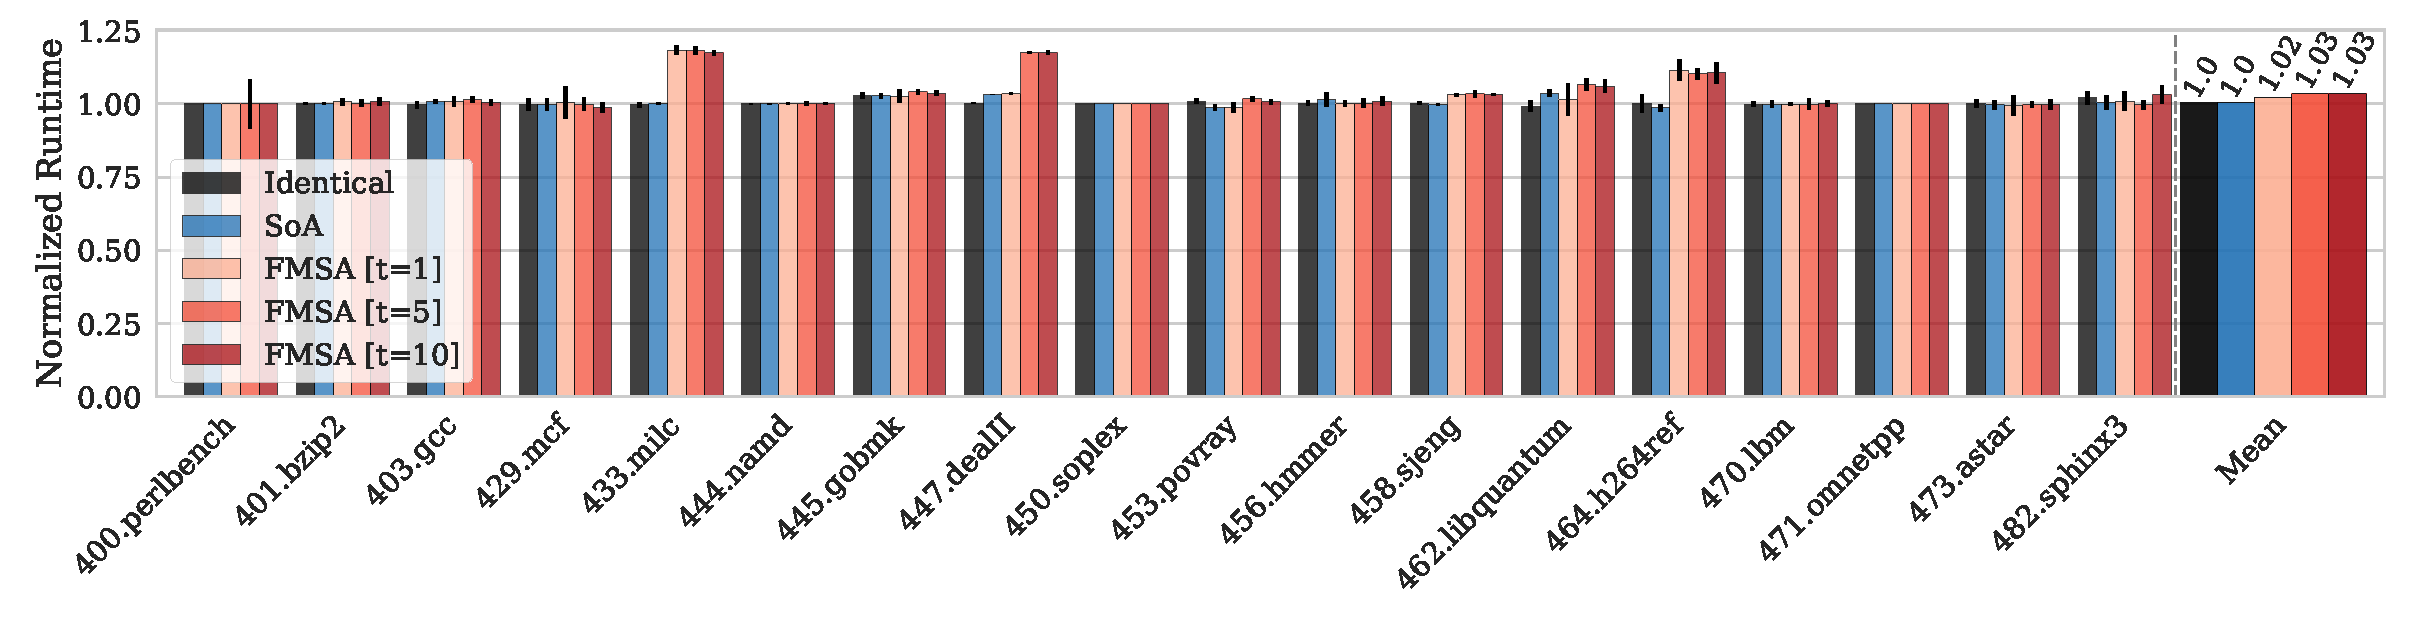
\includegraphics[width=\linewidth]{figs/runtime-impact.pdf}
  \vspace{-4ex}
  \caption{Runtime overhead on the Intel platform.}
  \label{fig:runtime-impact}
\end{figure*}

Unlike the other evaluated techniques, our optimization is a prototype
implementation, not yet tuned for compilation-time.
We believe that compilation-time can be further reduced with some additional engineering effort.
Nevertheless, by using our ranking infrastructure to target only the single most promising equivalent function for each function we examine,
we reduce compilation-time overhead by up to two orders of magnitude compared to the oracle.
This brings the average compile-time overhead to only 20\% compared to the baseline, while
still reducing code size almost as well as the oracle.
Depending on the acceptable trade-off between compilation-time overhead and code size,
the developer can change the exploration threshold to further shrink the binary or
accelerate compilation.

Figure~\ref{fig:compilation-time-breakdown} shows a detailed compilation-time
breakdown.
For each major step of the proposed optimization, we present the accumulated
time spent across the whole program.
To better understand the overhead of each one of the steps, we use
an exploration threshold of one ($t = 1$).
Because the ranking mechanism performs a quadratic operation on the number of
functions, computing the similarity between all pairs of functions, it is
expected that ranking would be amongst the most costly steps.
However, it is interesting to notice that the sequence alignment dominates most
of the compilation-time overhead, especially considering that this operation is
performed only once per function, when $t = 1$.
Although this operation is linear on the number of functions, the
Needleman-Wunsh algorithm~\cite{needleman70} is quadratic on the size of the
functions being aligned, both in time and space.
Unsurprisingly, the code generation is the third most costly step, which also
includes the time to optimize the merge of the parameters.
The remaining steps take, in total, a very small percentage of all the
compilation-time overhead.
This analysis suggests that optimizing the sequence alignment algorithm and
the ranking mechanism is key to reducing even further the overall
compilation-time overhead.

\vspace{-1ex}
\subsection{Performance Impact}


The primary goal of function merging is to reduce code size.
Nevertheless, it is also important to understand its impact on the programs'
execution time and the trade-offs between performance and code size reduction.
Figure~\ref{fig:runtime-impact} shows the normalized execution time.
Overall, our optimization has an average impact of about 3\% on programs' performance.
For most benchmarks, there is no statistically significant difference between
the baseline and the optimized binary. Only for \texttt{433.milc}, \texttt{447.dealII},
and \texttt{464.h264ref} there is a noticeable performance impact.

We focus on out worst result for \texttt{433.milc}. For an exploration threshold
value of one, we merge 58 functions. Through profiling, we discovered that a
handful of them are hot, that is they are frequently executed. If we prevent
these hot functions from merging, all performance impact is removed while still
reducing code size. Specifically, our original results showed a 5.11\% code size
reduction and an 18\% performance overhead. By avoiding merging hot functions,
we have an effectively non-existant performance impact and a code size reduction
of 2.09\%. While almost 9$\times$ less, this is still almost twice as good as
the state-of-the-art. As with the compilation overhead, this is a trade-off that
the developer can control.

%Note that the state-of-the-art has a reduction of only 1.09\% on this benchmark.
%If we can be more permissive, allowing some of the hot functions to be merged,
%we can have a code size reduction of 3.43\% while keeping the performance impact
%at about 4\%.

%However, \text{quantum\_gate1} is the largest function in the program,
%which means that this merge operation greatly contributes
%to the overall code-size reduction.
%Preventing this merge results in the code-size reduction dropping from 16\% to
%6.9\%, which is still a very significant code-size reduction compared to the
%other techniques that show no reduction on this particular benchmark.

%It is interesting to note that, for the 447.dealII benchmark, FMSA [t=1] has
%no extra impact than the state-of-the-art


%As a case study, we analyze the performance impact on the \text{462.libquantum}
%benchmark.
%After a detailed inspection of the program's execution with profiling
%information, we identified only two functions that contain the hottest basic
%blocks in the whole program.
%Hot basic blocks are determined based on the block frequencies recorded by
%instrumenting all basic blocks in the program~\cite{ball94}.
%The two hottest functions are: \text{quantum\_gate1} and
%\text{quantum\_decohere}.
%If we cross this information with the list of merged functions, we can confirm
%that the function \text{quantum\_gate1} is involved in a merge operation with
%a non-identical function.

%If, instead, we prevent this function of being merged, the performance
%impact goes away and we end up with a performance which is statistically
%equivalent to the baseline version.
%However, \text{quantum\_gate1} is the largest function in the program,
%which means that this merge operation greatly contributes
%to the overall code-size reduction.
%Preventing this merge results in the code-size reduction dropping from 16\% to
%6.9\%, which is still a very significant code-size reduction compared to the
%other techniques that show no reduction on this particular benchmark.
